\documentclass{standalone}
\usepackage{tikz}
\usetikzlibrary{patterns, positioning}


\begin{document}
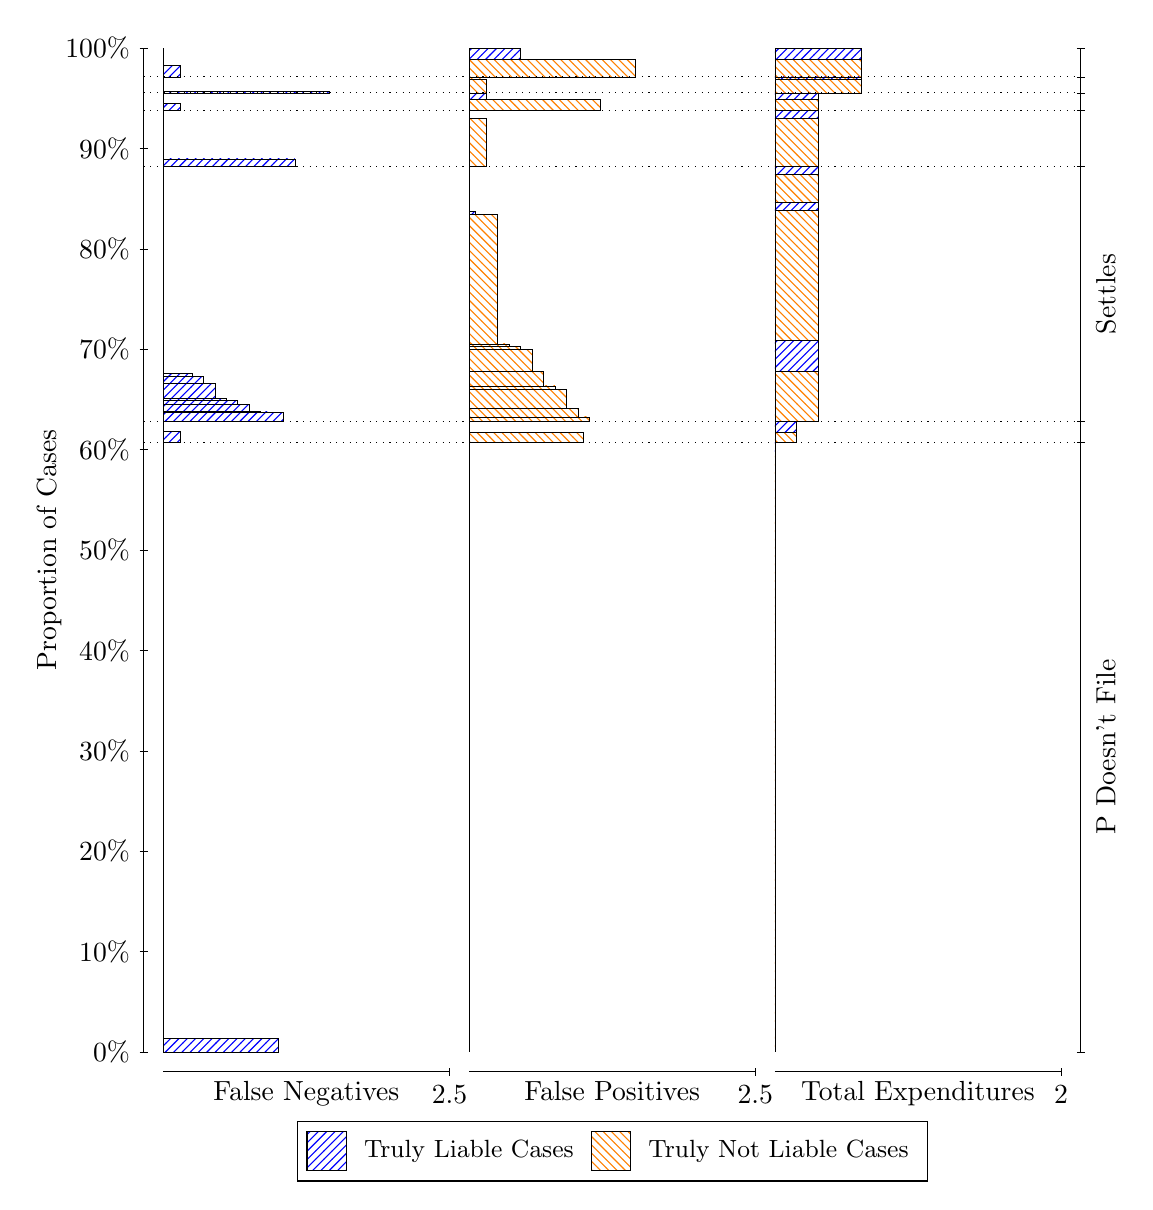
\begin{tikzpicture}
\draw[black, very thin] (1.5,1.75) -- (1.5,14.5);
\node[rotate=90, text=black, anchor=center] at (0.3, 8.125) {Proportion of Cases};
\draw[black, very thin] (1.45,1.75) -- (1.55,1.75);
\node[text=black, anchor=east] at (1.45, 1.75) {0\%};
\draw[black, very thin] (1.45,3.025) -- (1.55,3.025);
\node[text=black, anchor=east] at (1.45, 3.025) {10\%};
\draw[black, very thin] (1.45,4.3) -- (1.55,4.3);
\node[text=black, anchor=east] at (1.45, 4.3) {20\%};
\draw[black, very thin] (1.45,5.575) -- (1.55,5.575);
\node[text=black, anchor=east] at (1.45, 5.575) {30\%};
\draw[black, very thin] (1.45,6.85) -- (1.55,6.85);
\node[text=black, anchor=east] at (1.45, 6.85) {40\%};
\draw[black, very thin] (1.45,8.125) -- (1.55,8.125);
\node[text=black, anchor=east] at (1.45, 8.125) {50\%};
\draw[black, very thin] (1.45,9.4) -- (1.55,9.4);
\node[text=black, anchor=east] at (1.45, 9.4) {60\%};
\draw[black, very thin] (1.45,10.675) -- (1.55,10.675);
\node[text=black, anchor=east] at (1.45, 10.675) {70\%};
\draw[black, very thin] (1.45,11.95) -- (1.55,11.95);
\node[text=black, anchor=east] at (1.45, 11.95) {80\%};
\draw[black, very thin] (1.45,13.225) -- (1.55,13.225);
\node[text=black, anchor=east] at (1.45, 13.225) {90\%};
\draw[black, very thin] (1.45,14.5) -- (1.55,14.5);
\node[text=black, anchor=east] at (1.45, 14.5) {100\%};

\draw[black, very thin] (13.4,1.75) -- (13.4,14.5);
\draw[black, very thin] (13.35,1.75) -- (13.45,1.75);
\node[anchor=west] at (13.35, 1.75) {};
\draw[black, very thin] (13.35,9.4955) -- (13.45,9.4955);
\node[anchor=west] at (13.35, 9.4955) {};
\draw[black, very thin] (13.35,9.7593) -- (13.45,9.7593);
\node[anchor=west] at (13.35, 9.7593) {};
\draw[black, very thin] (13.35,12.993) -- (13.45,12.993);
\node[anchor=west] at (13.35, 12.993) {};
\draw[black, very thin] (13.35,13.709) -- (13.45,13.709);
\node[anchor=west] at (13.35, 13.709) {};
\draw[black, very thin] (13.35,13.93) -- (13.45,13.93);
\node[anchor=west] at (13.35, 13.93) {};
\draw[black, very thin] (13.35,14.133) -- (13.45,14.133);
\node[anchor=west] at (13.35, 14.133) {};
\draw[black, very thin] (13.35,14.5) -- (13.45,14.5);
\node[anchor=west] at (13.35, 14.5) {};

\draw[black, very thin, pattern color=blue, pattern=north east lines] (1.75,1.75) rectangle (3.2033,1.9249);
\draw[black, very thin, pattern color=orange, pattern=north west lines] (1.75,1.9249) rectangle (1.75,9.4955);
\draw[black, very thin, pattern color=blue, pattern=north east lines] (1.75,9.4955) rectangle (1.968,9.6322);
\draw[black, very thin, pattern color=orange, pattern=north west lines] (1.75,9.6322) rectangle (1.75,9.7593);
\draw[black, very thin, pattern color=blue, pattern=north east lines] (1.75,9.7593) rectangle (3.276,9.8685);
\draw[black, very thin, pattern color=blue, pattern=north east lines] (1.75,9.8685) rectangle (3.1307,9.8777);
\draw[black, very thin, pattern color=blue, pattern=north east lines] (1.75,9.8777) rectangle (2.9853,9.889);
\draw[black, very thin, pattern color=blue, pattern=north east lines] (1.75,9.889) rectangle (2.84,9.9707);
\draw[black, very thin, pattern color=blue, pattern=north east lines] (1.75,9.9707) rectangle (2.6947,10.026);
\draw[black, very thin, pattern color=blue, pattern=north east lines] (1.75,10.026) rectangle (2.5493,10.049);
\draw[black, very thin, pattern color=blue, pattern=north east lines] (1.75,10.049) rectangle (2.404,10.241);
\draw[black, very thin, pattern color=blue, pattern=north east lines] (1.75,10.241) rectangle (2.2587,10.325);
\draw[black, very thin, pattern color=blue, pattern=north east lines] (1.75,10.325) rectangle (2.1133,10.365);
\draw[black, very thin, pattern color=orange, pattern=north west lines] (1.75,10.365) rectangle (1.75,12.993);
\draw[black, very thin, pattern color=blue, pattern=north east lines] (1.75,12.993) rectangle (3.4213,13.093);
\draw[black, very thin, pattern color=orange, pattern=north west lines] (1.75,13.093) rectangle (1.75,13.709);
\draw[black, very thin, pattern color=blue, pattern=north east lines] (1.75,13.709) rectangle (1.968,13.795);
\draw[black, very thin, pattern color=orange, pattern=north west lines] (1.75,13.795) rectangle (1.75,13.93);
\draw[black, very thin, pattern color=blue, pattern=north east lines] (1.75,13.93) rectangle (3.8573,13.953);
\draw[black, very thin, pattern color=orange, pattern=north west lines] (1.75,13.953) rectangle (1.75,14.133);
\draw[black, very thin, pattern color=blue, pattern=north east lines] (1.75,14.133) rectangle (1.968,14.281);
\draw[black, very thin, pattern color=orange, pattern=north west lines] (1.75,14.281) rectangle (1.75,14.5);
\draw[black, very thin, pattern color=orange, pattern=north west lines] (5.6333,1.75) rectangle (5.6333,9.3206);
\draw[black, very thin, pattern color=blue, pattern=north east lines] (5.6333,9.3206) rectangle (5.6333,9.4955);
\draw[black, very thin, pattern color=orange, pattern=north west lines] (5.6333,9.4955) rectangle (7.0867,9.6226);
\draw[black, very thin, pattern color=blue, pattern=north east lines] (5.6333,9.6226) rectangle (5.6333,9.7593);
\draw[black, very thin, pattern color=orange, pattern=north west lines] (5.6333,9.7593) rectangle (7.1593,9.8158);
\draw[black, very thin, pattern color=orange, pattern=north west lines] (5.6333,9.8158) rectangle (7.014,9.9275);
\draw[black, very thin, pattern color=orange, pattern=north west lines] (5.6333,9.9275) rectangle (6.8687,10.168);
\draw[black, very thin, pattern color=orange, pattern=north west lines] (5.6333,10.168) rectangle (6.7233,10.21);
\draw[black, very thin, pattern color=orange, pattern=north west lines] (5.6333,10.21) rectangle (6.578,10.39);
\draw[black, very thin, pattern color=orange, pattern=north west lines] (5.6333,10.39) rectangle (6.4327,10.393);
\draw[black, very thin, pattern color=orange, pattern=north west lines] (5.6333,10.393) rectangle (6.4327,10.668);
\draw[black, very thin, pattern color=orange, pattern=north west lines] (5.6333,10.668) rectangle (6.2873,10.708);
\draw[black, very thin, pattern color=orange, pattern=north west lines] (5.6333,10.708) rectangle (6.142,10.743);
\draw[black, very thin, pattern color=orange, pattern=north west lines] (5.6333,10.743) rectangle (5.9967,12.387);
\draw[black, very thin, pattern color=blue, pattern=north east lines] (5.6333,12.387) rectangle (5.706,12.428);
\draw[black, very thin, pattern color=blue, pattern=north east lines] (5.6333,12.428) rectangle (5.6333,12.993);
\draw[black, very thin, pattern color=orange, pattern=north west lines] (5.6333,12.993) rectangle (5.8513,13.609);
\draw[black, very thin, pattern color=blue, pattern=north east lines] (5.6333,13.609) rectangle (5.6333,13.709);
\draw[black, very thin, pattern color=orange, pattern=north west lines] (5.6333,13.709) rectangle (7.3047,13.844);
\draw[black, very thin, pattern color=blue, pattern=north east lines] (5.6333,13.844) rectangle (5.8513,13.93);
\draw[black, very thin, pattern color=orange, pattern=north west lines] (5.6333,13.93) rectangle (5.8513,14.109);
\draw[black, very thin, pattern color=blue, pattern=north east lines] (5.6333,14.109) rectangle (5.6333,14.133);
\draw[black, very thin, pattern color=orange, pattern=north west lines] (5.6333,14.133) rectangle (7.7407,14.352);
\draw[black, very thin, pattern color=blue, pattern=north east lines] (5.6333,14.352) rectangle (6.2873,14.5);
\draw[black, very thin, pattern color=orange, pattern=north west lines] (9.5167,1.75) rectangle (9.5167,9.3206);
\draw[black, very thin, pattern color=blue, pattern=north east lines] (9.5167,9.3206) rectangle (9.5167,9.4955);
\draw[black, very thin, pattern color=orange, pattern=north west lines] (9.5167,9.4955) rectangle (9.7892,9.6226);
\draw[black, very thin, pattern color=blue, pattern=north east lines] (9.5167,9.6226) rectangle (9.7892,9.7593);
\draw[black, very thin, pattern color=orange, pattern=north west lines] (9.5167,9.7593) rectangle (10.062,10.393);
\draw[black, very thin, pattern color=blue, pattern=north east lines] (9.5167,10.393) rectangle (10.062,10.789);
\draw[black, very thin, pattern color=orange, pattern=north west lines] (9.5167,10.789) rectangle (10.062,12.434);
\draw[black, very thin, pattern color=blue, pattern=north east lines] (9.5167,12.434) rectangle (10.062,12.543);
\draw[black, very thin, pattern color=orange, pattern=north west lines] (9.5167,12.543) rectangle (10.062,12.893);
\draw[black, very thin, pattern color=blue, pattern=north east lines] (9.5167,12.893) rectangle (10.062,12.993);
\draw[black, very thin, pattern color=orange, pattern=north west lines] (9.5167,12.993) rectangle (10.062,13.609);
\draw[black, very thin, pattern color=blue, pattern=north east lines] (9.5167,13.609) rectangle (10.062,13.709);
\draw[black, very thin, pattern color=orange, pattern=north west lines] (9.5167,13.709) rectangle (10.062,13.844);
\draw[black, very thin, pattern color=blue, pattern=north east lines] (9.5167,13.844) rectangle (10.062,13.93);
\draw[black, very thin, pattern color=orange, pattern=north west lines] (9.5167,13.93) rectangle (10.607,14.109);
\draw[black, very thin, pattern color=blue, pattern=north east lines] (9.5167,14.109) rectangle (10.607,14.133);
\draw[black, very thin, pattern color=orange, pattern=north west lines] (9.5167,14.133) rectangle (10.607,14.352);
\draw[black, very thin, pattern color=blue, pattern=north east lines] (9.5167,14.352) rectangle (10.607,14.5);
\draw[black, dotted] (1.5,9.4955) -- (13.4,9.4955);
\draw[black, dotted] (1.5,9.7593) -- (13.4,9.7593);
\draw[black, dotted] (1.5,12.993) -- (13.4,12.993);
\draw[black, dotted] (1.5,13.709) -- (13.4,13.709);
\draw[black, dotted] (1.5,13.93) -- (13.4,13.93);
\draw[black, dotted] (1.5,14.133) -- (13.4,14.133);
\draw[black, very thin] (1.75,1.5) -- (5.3833,1.5);
\node[text=black, anchor=north] at (3.5667, 1.5) {False Negatives};
\draw[black, very thin] (5.3833,1.45) -- (5.3833,1.55);
\node[text=black, anchor=north] at (5.3833, 1.45) {2.5};

\draw[black, very thin] (5.6333,1.5) -- (9.2667,1.5);
\node[text=black, anchor=north] at (7.45, 1.5) {False Positives};
\draw[black, very thin] (9.2667,1.45) -- (9.2667,1.55);
\node[text=black, anchor=north] at (9.2667, 1.45) {2.5};

\draw[black, very thin] (9.5167,1.5) -- (13.15,1.5);
\node[text=black, anchor=north] at (11.333, 1.5) {Total Expenditures};
\draw[black, very thin] (13.15,1.45) -- (13.15,1.55);
\node[text=black, anchor=north] at (13.15, 1.45) {2};

\node[text=black, centered, rotate=90] at (13.72, 5.6227) {P Doesn't File};

\node[text=black, centered, rotate=90] at (13.72, 11.376) {Settles};





\draw (7.449999999999999,1.5) node[draw=none] (baseCoordinate) {};
\begin{scope}[align=center]
        \matrix[scale=0.5, draw=black, below=0.5cm of baseCoordinate, nodes={draw}, column sep=0.1cm]{
            \node[rectangle, draw, minimum width=0.5cm, minimum height=0.5cm, pattern color=blue, pattern=north east lines] {}; &
            \node[draw=none, font=\small, text=black] (B) {Truly Liable Cases}; &
            \node[rectangle, draw, minimum width=0.5cm, minimum height=0.5cm, pattern color=orange, pattern=north west lines] {}; &
            \node[draw=none, font=\small, text=black] (B) {Truly Not Liable Cases}; \\
            };
\end{scope}

\end{tikzpicture}
\end{document}